%%%%%%%%%%%%%%%%%%%%%%%%%%%%%%%%%%%%%%%%%%%%%%%%%%%%%%%%%%%%%%%%%%%%%%%%
%                                                                      %
%     File: Thesis_Results.tex                                         %
%     Tex Master: Thesis.tex                                           %
%                                                                      %
%     Author: Andre C. Marta                                           %
%     Last modified:  2 Jul 2015                                      %
%                                                                      %
%%%%%%%%%%%%%%%%%%%%%%%%%%%%%%%%%%%%%%%%%%%%%%%%%%%%%%%%%%%%%%%%%%%%%%%%

\chapter{Results}
\label{chapter:results}

In this chapter, experimental tests for Darknet lite, the DeepVersat software simulator, and the new API functions are presented.
In Section \ref{section:DNNDescription}, the DNN description of the Darknet Reference Model is translated. 
Afterward, in section \ref{section:simtest}, the simulator is tested and the results are checked between a CPU-only run and the simulator run. 
Finally, in section \ref{section:testgencov}, test cases for matrix
multiplication and generic convolution are presented. The convolution test case
features several hardware configurations, which test different simulation
scenarios more thoroughly while using a randomized input and kernel. 

The tests were executed on a 64-bit machine, with an AMD Ryzen 7 5800H Processor
and 16GB of RAM running Windows 11, version 22H2, WSL 2.0 with the image of
Ubuntu 20.04. The compiler used is G++ version 9.4.0.

%%%%%%%%%%%%%%%%%%%%%%%%%%%%%%%%%%%%%%%%%%%%%%%%%%%%%%%%%%%%%%%%%%%%%%%%%


\section{Compiling DNN Description}
\label{section:DNNDescription}

The Darknet Reference Model is a 15-layer CNN that is designed to have similar performance to AlexNet\cite{alexnet} while using 1/10th the parameters. 
It achieves top-1 accuracy of 61.1\% and a top-5 accuracy of 83\%. In a CPU-only scenario, it takes 0.14s per image. When using the CUDA API, it drops to 2.9ms per image.

To compile the CNN, we run the DNN compiler, which uses the darknet parser to write the configurations for Darknet lite, as mentioned in \ref{chapter:Darknet}.

\lstinputlisting[label=DNNcompiler,language=C++,frame=single,breaklines=true,firstline=1,lastline=52,caption= Darknet Reference Model configuration file for the first four layers]{./Code/darknet.cfg}

When running the DNN compiler, it checks to see if every layer in the description is implemented in Darknet lite, giving the terminal output in \ref{figure:DNNcompiler}.

\begin{figure}[!htbp]
    \centering
    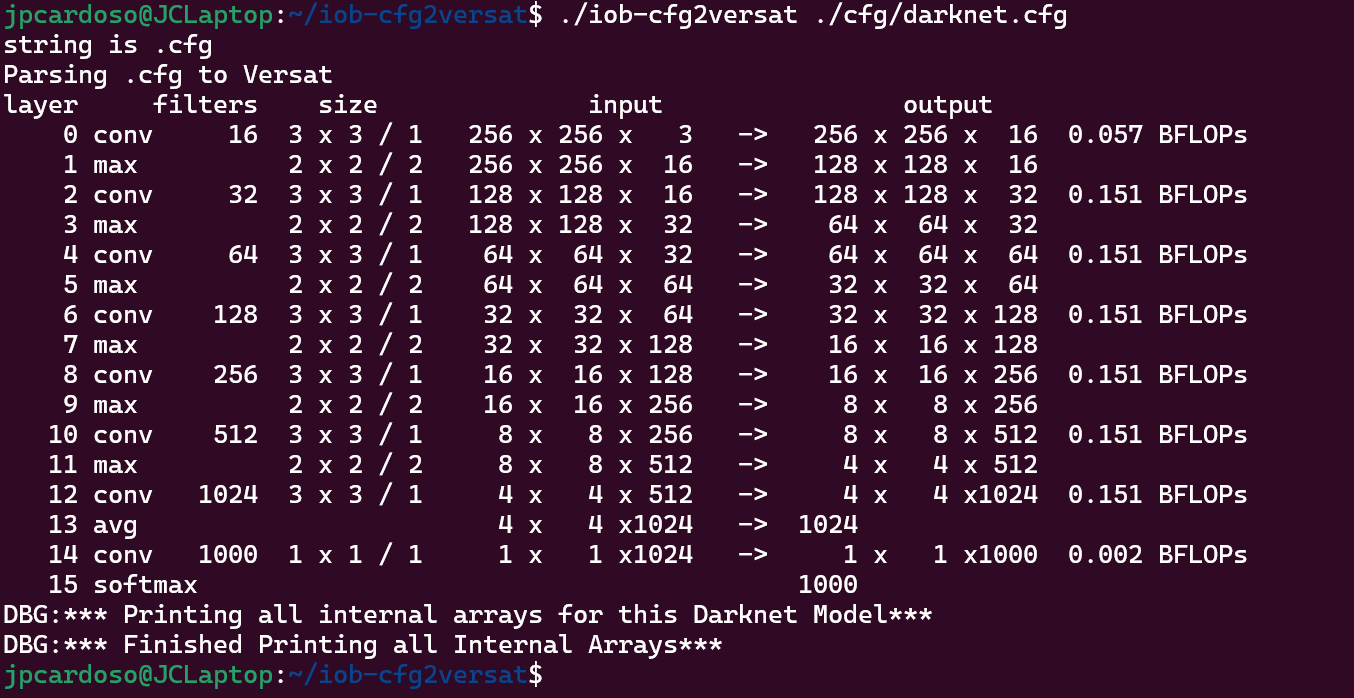
\includegraphics[width=\textwidth]{Figures/darknet1.png}
    \caption{DNN Compiling of the Darknet Reference Model}
    \label{figure:DNNcompiler}
\end{figure} 

%%%%%%%%%%%%%%%%%%%%%%%%%%%%%%%%%%%%%%%%%%%%%%%%%%%%%%%%%%%%%%%%%%%%%%%%


\section{Simulator Testing}
\label{section:simtest}

To test the simulator, a test program was created that will create a random input matrix of 5x5
with a kernel size of 3. For each Stage defined in the headers file, a channel will be added, and the result of the convolution will propagate through the stages.

To be more specific, in the beginning, the configurations of the VIs are written to transfer the data
from the program to Versat. The data uses the rand() function with seed using current time
so the result is different every time. Both the input matrix and kernel map are randomized.
The former value varies from -25 to 25, while the kernel varies from -5 to 5. Using the data, 
we calculate the result of the convolution in the CPU. Afterward, the configuration for the Bias mem
is done, and then stage by stage, the configuration of the VI, MAC, and ALU is done. Finally, the
configuration of the VO is written.


\lstinputlisting[label=testbench1,language=C++,frame=single,breaklines=true,firstline=298,lastline=341,caption=Loading Data into Deep Versat using CMem FU]{./Code/testbench.cpp}


\begin{figure}[!htbp]
    \centering
    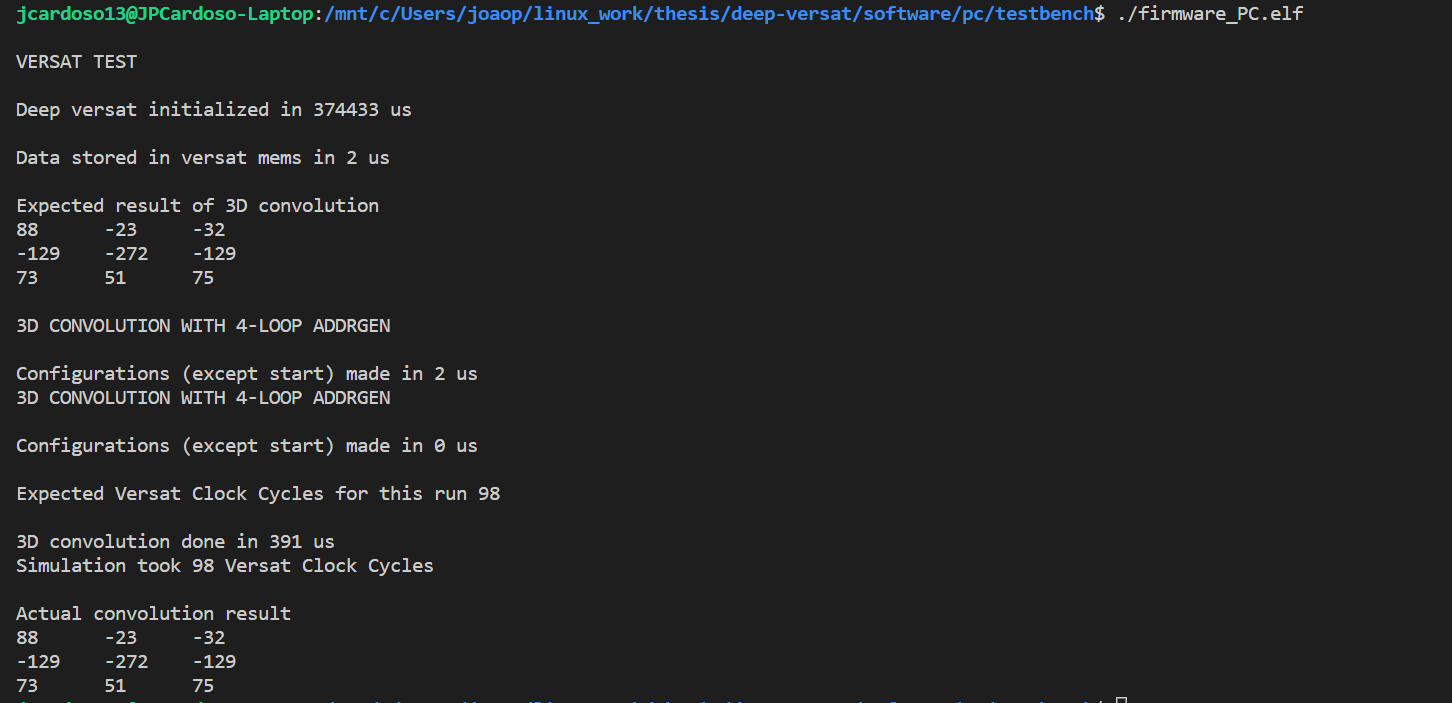
\includegraphics[width=\textwidth]{Figures/test1.png}
    \caption{Simulator test output in terminal}
    \label{figure:test1}
\end{figure} 

The estimated iterations needed are the following:

\[ Est=Delay+Iter_2*Per_2*Iter_1*Per_1\]

Where these are the AGU configurations of the VO where the results are written. The Delay is accumulated
through the several stages by adding two due to the MACs and ALUs.

\lstinputlisting[label=testbench2,language=C++,frame=single,breaklines=true,firstline=371,lastline=437,caption=Writting the configurations of DeepVersat using API v1]{./Code/testbench.cpp}


%%%%%%%%%%%%%%%%%%%%%%%%%%%%%%%%%%%%%%%%%%%%%%%%%%%%%%%%%%%%%%%%%%%%%%%%
\section{Testing the new API}
\label{section:testgencov}

In this section, the same method for the previous test file is made. 
While the previous one relies on using API v1 for the configuration, these test benches
run the new API. 

\subsection{Test File for Matrix Multiplication}

\begin{figure}[!htbp]
    \centering
    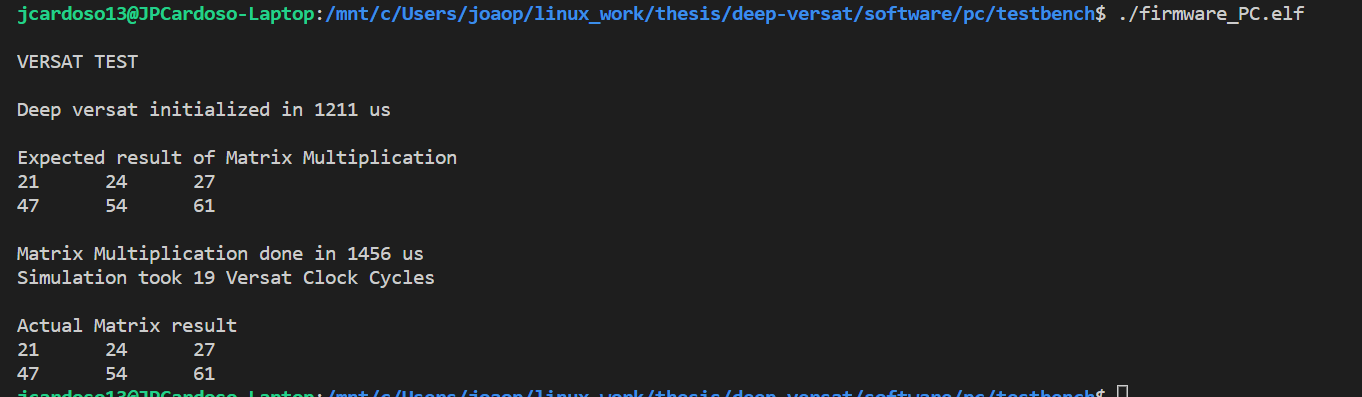
\includegraphics[width=\textwidth]{Figures/test2.png}
    \caption{Matrix Multiplication Test File Outputs}
    \label{figure:test2}
\end{figure}

The Matrix Multiplication is a quite simple program. The only thing needed is an instance
Versat, run versat\_init(), create the matrixes, and then use the function matrix\_multiplication()
The data is also computed in the CPU result to verify the output, which can be found in
figure \ref{figure:test2}. In Listing\ref{testbench3}, the code of the test file is presented.

\lstinputlisting[label=testbench3,language=C++,frame=single,breaklines=true,firstline=22,lastline=91,caption=Writting the configurations of DeepVersat using API v2 for Matrix Multiplication]{./Code/testMatrixMult.cpp}


\subsection{Test File for Generic Convolution}

Using the same method on the previous test benches, the following Convolution Layer was used
with several Versat Configurations.

\begin{table}[!htpb]
    \centering
    \begin{tabular}{ll}
    \hline
    \textbf{CNN Variable} & \textbf{Value}        \\ \hline
    Kernel Size            & 2                 \\
    Channels            & 2                       \\
    Number of Kernels            & 2                       \\
    Input Height                  & 12                        \\
    Input Width                & 12                  \\
    Stride              & 1                     \\
    Out Width               & 11                      \\
    Out Height            & 11  \\
    Out Channels                   & 2                     \\ \hline
    \end{tabular}
    \label{table:convInput}
    \caption{CNN Layer on the test file}
\end{table}

With this layer, Figure~\ref{figure:test3} has the output result of the generic convolution test file.
For this specific Versat hardware configuration, the number of iterations needed is 711 using three  Datapaths.

\begin{figure}[!htbp]
    \centering
    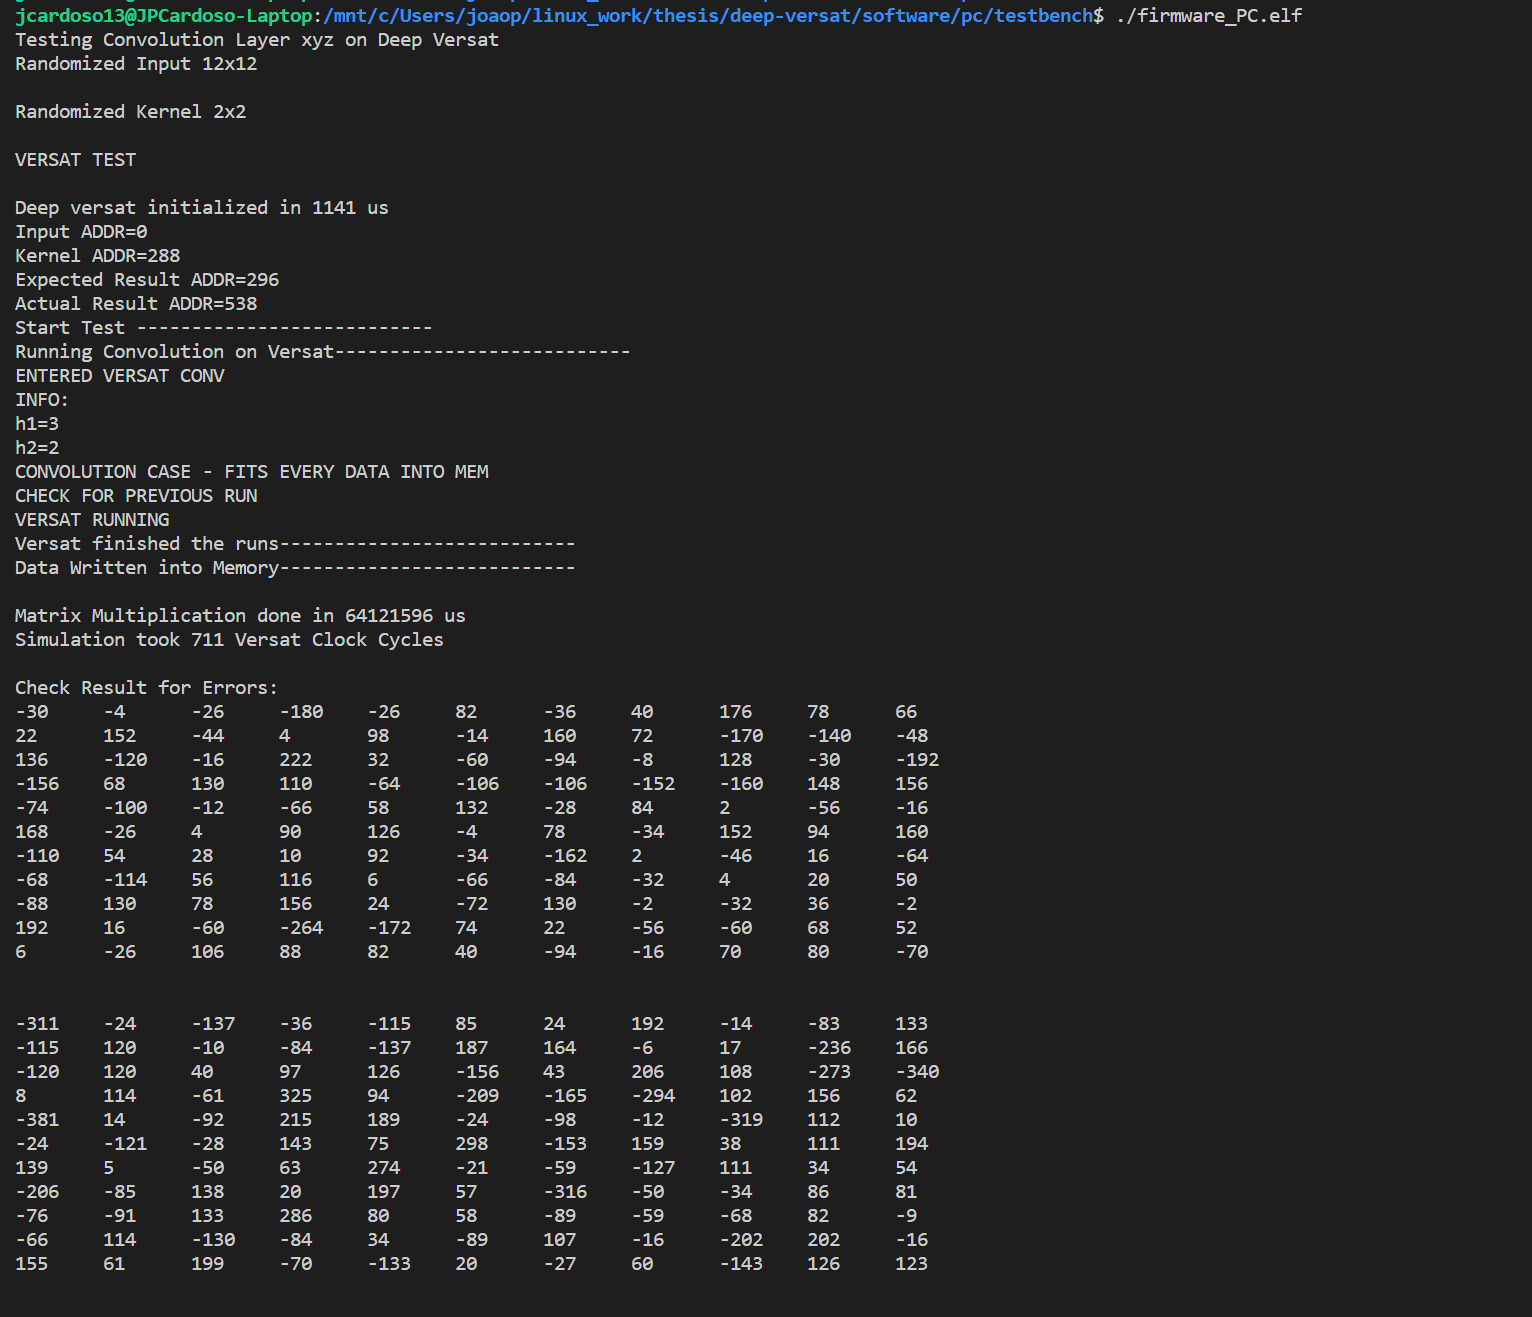
\includegraphics[width=\textwidth]{Figures/test3.png}
    \caption{Generic Convolution test file Outputs}
    \label{figure:test3}
\end{figure}

In Table \ref{table:Iterations}, the different Datapath numbers and how it affects performance.
A datapath is a combination of 1 VI, 1 MAC, and 1 VO. So the lower number in the Versat configuration file
decides the number of valid datapaths. Of course, VI needs +1 in numbers more than the functional units due to the Kernel memory.
\newpage
\begin{table}[!htpb]
    \centering
    \begin{tabular}{ll}
    \hline
    \textbf{Number of Datapaths} &  \textbf{Iterations}        \\ \hline
    1          & 1943                 \\
	2          & 1063                 \\
	3          & 711                 \\
	4          & 535                 \\
	6          & 359                 \\
	8          & 359                 \\
	11          & 183                 \\
	16          & 183                 \\
    22            & 183                       \\  \hline
    \end{tabular}
    \label{table:Iterations}
    \caption{CNN Layer on the test file with several Versat hardware configurations}
\end{table}

The reason for these results is quite simple. In total, 11 output lines are divided
by the datapaths. When the division is not a whole number, the remainder gets distributed
by available datapaths. The consequence of this, when changing from six to eight datapaths, the performance
doesn't get any better. Datapath zero will have to run twice to (2 lines) while Datapath 8 will run one line.
To increase the performance further, the output channels would have to be divided through more datapaths.

Finally, in Listing \ref{testbench4}, we present the code for running the generic convolution test, showcasing the reduced code complexity compared to that in Section \ref{section:simtest}. The majority of the code pertains to establishing the testing environment and verifying the results, highlighting the simplified development process for the developer.

\lstinputlisting[label=testbench4,language=C++,frame=single,breaklines=true,firstline=22,lastline=182,caption=Writting the configurations of DeepVersat using API v2 for Generic Convolution]{./Code/testConvolution.cpp}
